%
% File acl2015.tex
%
% Contact: car@ir.hit.edu.cn, gdzhou@suda.edu.cn
%%
%% Based on the style files for ACL-2014, which were, in turn,
%% Based on the style files for ACL-2013, which were, in turn,
%% Based on the style files for ACL-2012, which were, in turn,
%% based on the style files for ACL-2011, which were, in turn, 
%% based on the style files for ACL-2010, which were, in turn, 
%% based on the style files for ACL-IJCNLP-2009, which were, in turn,
%% based on the style files for EACL-2009 and IJCNLP-2008...

%% Based on the style files for EACL 2006 by 
%%e.agirre@ehu.es or Sergi.Balari@uab.es
%% and that of ACL 08 by Joakim Nivre and Noah Smith

\documentclass[11pt]{article}
\usepackage{acl2015}
\usepackage{times}
\usepackage{url}
\usepackage{latexsym}
\usepackage{color, listings, graphicx, float, booktabs, multirow, outlines,changepage, fancybox, amsmath,enumitem, outlines}
\graphicspath{{./figures/}}

%\setlength\titlebox{5cm}

% You can expand the titlebox if you need extra space
% to show all the authors. Please do not make the titlebox
% smaller than 5cm (the original size); we will check this
% in the camera-ready version and ask you to change it back.

\definecolor{codegreen}{rgb}{0,0.6,0}
\definecolor{codegray}{rgb}{0.5,0.5,0.5}
\definecolor{codepurple}{rgb}{0.58,0,0.82}
\definecolor{backcolour}{rgb}{0.95,0.95,0.92}
 
\lstdefinestyle{mystyle}{
    backgroundcolor=\color{backcolour},   
    commentstyle=\color{codegreen},
    keywordstyle=\color{magenta},
    numberstyle=\tiny\color{codegray},
    stringstyle=\color{codepurple},
    basicstyle=\footnotesize,
    breakatwhitespace=false,         
    breaklines=true,                 
    captionpos=b,                    
    keepspaces=true,                 
    numbers=left,                    
    numbersep=5pt,                  
    showspaces=false,                
    showstringspaces=false,
    showtabs=false,                  
    tabsize=2
}
 
\lstset{style=mystyle}



\title{Instructions for ACL-2015 Proceedings}

\begin{document}
\begin{center}
	\textbf{\large{A Simple CUDA Neural Network}}\\
	Kyle Salitrik (kps168), Tomoki Takasawa (tmt5336)
\end{center}
\begin{abstract}
		
\end{abstract}

\section{Credits}
Images throughout the forward propgation section were obtained from: neuralnetworksanddeeplearning.com/chap1.html

\section{Introduction and Objectives}
This program is designed to identify hand written numbers (0 ~ 9) by neural network digit classification technique. Generally, this technique requires enourmous amuont of run time. For training process, it calculates 5 matrix multiplications, 2 matrix subtractions, and 5 elemnt-wise vector operations. For verification, it requires 2 matrix multiplications and 2 element-wise operations for sigmoid function. In the case of all of the operations listed, the matrices and vectors are all densely populated. We decided to approach this problem by processing these operations in parallel on NVDIA's GPU processors. 

\section{Neural Network Structure}
All figures in this section were obtained from the source credited in section 1. The general purpose of the neural network is identifying handwritten digits 28x28 in size. An example of the handwritten data is shown below. This dataset, called MNIST, is commonly used to benchmark neural network performance. The handwriting samples were obtained by the U.S. National Institute of Standards and Technology (NIST) from both census workers and high school students. This data is divided into 50,000 training samples, 10,000 test samples, and 10,000 validation samples.

\begin{figure}[H]
	\centering
	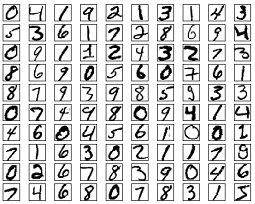
\includegraphics[width=.4\textwidth]{mnist_100_digits.png}
	\caption{MNIST Data}
\end{figure}

Although it will be explained in the next section in detail, it is important to know that each neuron within the network will output a value between 0 and 1. This value is bound by what is called the activation function of the neuron. The input to the neural network was a matrix of 28x28 reshaped into a single column vector of size 784, with each neuron (vector element) representing a single pixel in the image. Initially the data is defined by a value of 0-127 for pixel intensity, but it is then bound to a value between 0 and 1 by simply dividing each element by 127. 

The hidden (or second) layer size of 128 neurons was arbitrarily chosen. While the objective was to train a simple neural network with only one hidden layer. A deep neural network may consist of a network with two or more hidden layers, typically each layer will reduce in size with each step forward in the network closer to the desired output layer size. These hidden layer sizes can be tuned (known as meta-parameters) in order to change the behavior of the network. The final (output) layer of the network consists of 10 neurons, with each neuron (0 through 9) representing the corresponding numerical digit. This format results in a vector similar to the following:
\begin{center}
	$[ 0, 0, 0, 1, 0, 0, 0, 0, 0, 0, 0 ]$\\
\end{center}
This representation is known as a 1-hot format, where the element that has a value of 1 indicates the corresponding digit as true. Referencing the above example, it represents the digit 3 (as element 3 has a value of 1). With regard to the output layer, the neuron with the highest value is chosen as the "answer" by the network. The structure for the neural network was as follows:
\begin{itemize}[noitemsep,nolistsep]
	\item Layer 1 (input): 784 neurons
	\item Layer 2 (hidden layer): 128 neurons
	\item Layer 3 (output): 10 neurons
\end{itemize}


\section{Forward Propogation}
The behaivor of the neural network is defined by a function chosen by the network implementor. When a set of inputs are passed into a neuron layer (pictured below), each neuron in the layer computes its activation using this predetermined function. For the case of this assignment (and most simple neural networks), the sigmoid function was used. The sigmoid function helps us to bind the output from our neurons between 0 and 1 because we are looking for a (mostly) boolean answer: true or false for identifying a digit. This is where a significant portion of our computational cost comes from, as it includes a floating point exponential function, division and addition.
\begin{align}
	\sigma(z) & = \frac{1}{1 + e^{-z}} & \text{Sigmoid Function} 
\end{align}

\begin{figure}[H]
	\centering
	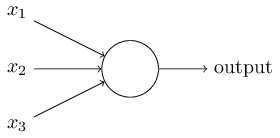
\includegraphics[scale=.5]{nn0.png}
	\caption{Neuron Diagram}
\end{figure}

In our case, we use a densely connected neural network where every neuron in a layer is connected to every neuron in the following layer. It is useful to know that other types of layer relationships do exist such as sparsely connected layers, but are not explored here. These connections are defined by weight matrices where each element represents the connection from neuron A in layer L to neuron B in layer $L+1$.

\begin{figure}[H]
	\centering
	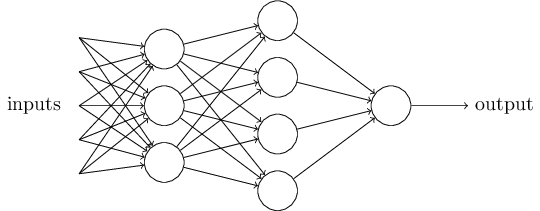
\includegraphics[width=.45\textwidth]{nn1.png}
	\caption{Neuron Diagram}
\end{figure}

The majority of the computational costs arise from the vector-matrix multiplication between these dense weight matrices and the activations of the previous neurons. Each weight matrix is initalized to a random set of values and is adjusted during the final step (gradient descent) after each iteration through the network. In the following equations, $a^{(l)}$ represents the activation of layer $l$ and $\theta^{(l)}$ represents the weights between $a^{(l)}$ and $a^{(l+1)}$
 
To compute a full pass of forward propogation, we must compute the following equations:
\begin{align*}
	z^{(2)} & = a^{(1)}*\theta^{(1)T} \\
	a^{(2)} & = \sigma\{z^{(2)}\}     \\
	z^{(3)} & = a^{(2)}*\theta^{(2)T} \\
	a^{(3)} & = \sigma\{z^{(3)}\}
\end{align*}

For our neural networks, the following are the weight matrix sizes:
\begin{itemize}[noitemsep,nolistsep]
	\item Weight Matrix 1: 128x784 elements
	\item Weight Matrix 2: 10x128 elements
\end{itemize}

At this point, the forward propogation has computed the estimated answer to a given input. Next, the result is evaluated in backpropogation which prepares for adjusting the weights to be more accurate.

\section{Backward Propogation}
The second step in training a neural network, as stated previously, is called backpropogation. This step evaluates the error in each layer's activations. This information can be used simply as a metric evaluated by a defined cost function (not used for our purposes) or can be used to adjust the weights through various methods. The validation data is typically used for computing the cost function.

The first step in backpropogation is to evaluate how far off the network was from the expected result. To do this the following value is caluclated, where $y$ is the known answer in one-hot format:
\begin{align*}
	\delta^{(3)} & = a^{(3)} - y
\end{align*}

Because we know the error of the last layer, we can calculate the error contributed by each previous layer -- excluding the input layer -- by the following implicit function:
\begin{align}
	\delta^{(l)} & = \widehat{\delta}^{(l+1)}\widehat{\Theta}^{(l)} \odot \sigma'(z^{(l)})
\end{align}

In the previous equation $\odot$ represents the Hadamard product (element wise multiplication) for vectors, and $\sigma'(z)$ is the derivative of the sigmoid function:

\begin{align}
	\sigma'(z) & = & \sigma(z) \odot (1 - \sigma(z))
\end{align}

Knowing these functions, we must only evaluate (2) for the following, as we only have one more hidden layer:
\begin{align*}
	\delta^{(2)} & = \widehat{\delta}^{(3)}\widehat{\Theta}^{(2)} \odot \sigma'(z^2)
\end{align*}

However, this is an extremely computationally costly function, including a floating point vector-matrix multiply, floating point subroutines, divides, additions, and multiplications, which is why parallel computing is very tempting to use. At this point we are ready to move on to the final step of training the network: gradient descent.

\section{Gradient Descent}
Gradient descent computes the gradient of the weights for each weight matrix and is usually adjusted by 1 divided by the number of data samples ($m$). The weight matrices are adjusted by these gradients in order to find a local minima. Before proceeding it is worth noting that gradient descent is not the ONLY method for training a network's weights, nor is it the best. One common pitfall includes overshooting the minima and ending up in a divergent inflation of the weights. This is why the 1/m adjustment is applied to the gradient.

The following equation is the computation for the gradient of each weight matrix:
\begin{align}
	\nabla\frac{\partial J}{\partial\Theta^{(l)}} & = \frac{1}{m} \delta^{(l+1)T}*a^{(l)}
\end{align}

For the investigated network, the following gradients were computed after each forward propogation for each data example (image).
\begin{align*}
	\nabla^{(1)} & = \frac{1}{m} \delta^{(2)T}*a^{(1)}\\
	\nabla^{(2)} & = \frac{1}{m} \delta^{(3)T}*a^{(2)}
\end{align*} 

The final step in gradient descent is to adjust the weight matrices by the gradients:
\begin{align*}
	W1 &:= W1 - \nabla^{(1)} \\
	W2 &:= W2 - \nabla^{(2)}
\end{align*}

\section{Testing the Network}
Typically to train the network, the training data is cycled through in its entirety (known as one epoch) and then shuffled to be run for another epoch. The number of epochs is dependent on the accuracy desired and the time allowed for computation. To test the network after the training epochs, the test data is run through the network and the number of correct predictions out of the number of total testing examples is reported to determine the networks accuracy. Using more advanced methods, networks for the MNIST data can obtain $>90\%$ performance.

\section{Performance}
For the network employed, we were only able to successfully run training with $\approx 20,000-30,000$ training samples and $10,000$ testing samples due to restrictions on the ACI-I cluster. One major issue encountered with the ACI-I nodes was that one person is capable of utilizing the entire CUDA device at once, so there was no way to guarantee obtaining enough memory for the computations. However on this limited subset of training data, the network was able to identify nearly 1/5th of the training data presented correctly.

All things considered, using these standard methods with the full training samples and multiple (5-10) epochs typically results in a near 80\% accuracy in digit identification, so 20\% using only 20,000 samples is quite good. This is considering that if a network is trained using all 50,000 samples 10 times each, that results in a total of 500,000 iterations through backpropogation and gradient descent in order to train the network, so using only 4\% of the number of training iterations to obtain nearly 25\% of the performance is promising.

\section{Alternate Approaches and Future Work}
One alternate method is to train using the entire 50,000 samples at one time instead of iterating through forward propogation for each sample individually. It is possible that using this method with CUDA may improve performance significantly. It was not attempted in order to stay true to a traditional network training scenario. Other future work would include making the computations more memory efficient.

\section{Code Function Explanations}
\begin{outline}
	\setlength\itemsep{0em}
	\1 setVectorSize:
		\2 This function sets the vector size and store them in struct, \_vSize.
	\1 setMatrixSize:
		\2 This function sets the matrix size and store them in struct, \_matrixSize.
	\1 VectorInitCUDA / MatrixInitCUDA:
		\2 This function allocates memory in GPU, and copy the value from local machine.
	\1 VectorAdditionKernel:
		\2 CUDA Kernel to add two vectors
	\1 VectorHadmardKernel:
		\2 CUDA Kernel to compute the Hadamard product of two vectors
	\1 VectorDotProduct:
		\2 CUDA Kernel to compute the dot product of two vectors
	\1 VectorSigmoid:
		\2 CUDA Kernel that computes the sigmoid function for each item in a vector
	\1 VectorSigmoidDerivative:
		\2 CUDA Kernel that computes the sigmoid function derivative for each item in a vector
	\1 MatrixAddKernel:
		\2 CUDA Kernel to add or subtract two matrices
	\1 MatrixHadamardKernel:
		\2 CUDA Kernel to compute the Hadamard product of two matrices
	\1 MatrixSigmoidMatrix:
		\2 CUDA Kernel that computes the sigmoid function for each item in a matrix
	\1 SigmoidDerivative:
		\2 CUDA Kernel that computes the sigmoid function derivative for each item in a matrix
	\1 RunVectorKernel:
		\2 This function allocate and initialize memory in GPU and call functions for vector operations, VectorAdditionKernel, VectorHadmardKernel, VectorDotProduct, VectorSigmoid, VectorSigmoidDerivative functions. Then, it frees memory.
	\1 MatrixMultiplyCUBLAS:
		\2 This allocates and initialize memory in GPU and perform matirix multiplication by calling cublasSgemm, which is part of NVIDIA's library. Then, it frees memory.
	\1 RunMatrixKernel:
		\2 This function allocate and initialize memory in GPU and calls functions for matrix operations, MatrixAddKernel, MatrixHadamardKernel, MatrixSigmoidMatrix, and SigmoidDerivative. Then, it frees memory.
	\1 runTest:
		\2 This is a test function that was used for testing the kernels before the network was implemented. 
	\1 main: 
		\2 It allocates memory for activation vectors, pre-sigmoid intermediary vectors, weight matrices, one-hot result vectore, error vectors, and error gradients in local machine, and initialize them. Then, it calls RunVectorKernel and MatrixMultiplyCUBLAS

\end{outline}


% include your own bib file like this:
%\bibliographystyle{acl}
%\bibliography{acl2015}

\begin{thebibliography}{}
		
	\bibitem[\protect\citename{Gusfield}1997]{Gusfield:97}
	Michael Nielsen.
	\newblock 2017.
	\newblock {\em Neural Networks and Deep Learning Book}.
	\newblock neuralnetworksanddeeplearning.com.
		
\end{thebibliography}

\newpage
\onecolumn
\section*{Code Appendix}
\lstinputlisting[language=C]{../src/cuda_nn.cu}

\end{document}